
% File acl2010.tex
%
% Contact  jshin@csie.ncnu.edu.tw or pkoehn@inf.ed.ac.uk
%%
%% Based on the style files for ACL-IJCNLP-2009, which were, in turn,
%% based on the style files for EACL-2009 and IJCNLP-2008...

%% Based on the style files for EACL 2006 by 
%%e.agirre@ehu.es or Sergi.Balari@uab.es
%% and that of ACL 08 by Joakim Nivre and Noah Smith

\documentclass[12pt]{article}
\usepackage{acl2010}
\usepackage{times}
\usepackage{url}
\usepackage{amsmath}
%\setlength\titlebox{6.5cm}    % You can expand the title box if you
% really have to
% \usepackage[brazilian]{babel}
\usepackage[brazil]{babel}
\usepackage[utf8]{inputenc}
\usepackage{graphicx}% Include figure files
\selectlanguage{brazil}

\title{Aprendizado Semi-Supervisionado Baseado em Grafos}

\author{Renato Fabbri\\
Universidade de São Paulo, São Carlos, São Paulo, Brazil\\
{renato.fabbri@gmail.com}\\
{\tt Junho de 2010}}

\begin{document}

\maketitle
\begin{abstract}
Neste trabalho abordamos em especial dois métodos de aprendizado semi-supervisionado que se baseiam em grafos. Primeiramente apresentamos brevemente o assunto de aprendizado semi-supervisionado. Depois expomos, também brevemente, o que vem a ser grafos e redes complexas. Na sequência explicitamos os dois métodos que julgamos representativos do aprendizado semi-supervisionado com grafos, a saber o método de propagação de rótulos e o método de mincut. Finalizamos com algumas palavras sobre os dois métodos e suas utilidades e pontos fracos.
\end{abstract}

\section{Introdução}

\subsection{Aprendizado Semi-Supervisionado}
O \emph{aprendizado semi-supervisionado} (ASS) visa o aprendizado a partir da utilização tanto dos objetos rotulados quanto dos não rotulados. São exemplos de ASS a \emph{classificação semi-supervisionada} (CSS) e a \emph{clusterização forçada}. Este trabalho é um apanhado sobre CSS em grafos que é como geralmente é entendido o ASS com grafos.

O nome "semi-supervisionado" vem do fato de que os dados utilizados para o aprendizado está entre os dados utilizados no aprendizado supervisionado e não supervisionado\footnote{No aprendizado \emph{supervisionado} são utilizados somente dados rotulados. No aprendizado \emph{não supervisionado} são utilizados somente dados não rotulados.}.

Podemos comparar a CSS ao processo de uma criança que entende o que é um animal através de alguns exemplos dados pelos adultos e de outros vários que ela mesma observa. Ou seja, para o aprendizado do que é (e o que não é) um animal, ela utiliza tanto o conhecimento sobre os animais que contaram para ela que é um animal quanto o conhecimento sobre outros seres que não falaram para ela o que é.

Um grande atrativo dos métodos de ASS é que ele pode ajudar a contornar o fato de que os objetos rotulados podem ser custosos. Comumente necessitam de um humano especializado para rotulá-los, outras vezes necessitam de equipamentos, condições ou processamentos especiais. Muitas vezes é simplesmente impossível obter novos objetos rotulados. Já os objetos não rotulados são geralmente imediatos e abundantes, podendo ser utilizados pelo ASS de imediato.

Uma distinção importante que se faz é quanto ao ASS \emph{indutivo} e o ASS \emph{transdutivo}. O ASS indutivo se assemelha ao aprendizado transdutivo. A diferença entre ambos é que o aprendizado transdutivo é otimizado para tratar somente os objetos utilizados para o treinamento, enquanto o ASS indutivo trata de objetos não presentes na fase de treinamento.

Dados não rotulados podem ajudar de diversas formas, em especial quando as diferentes classes se mostram clusterizadas. Na Figura \ref{fig:help} é explicitado esquematicamente a forma com que os dados não rotulados podem auxiliar a determinar uma fronteira de decisão mais pertinente. Embora este seja o comportamento natural mais comum, devemos notar que o contrário também ocorre e que neste caso o princípio da clusterização das classes semelhantes pode nos levar a resultados enganosos. A Figura \ref{fig:nhelp} demonstra este caso no qual o critério de clusterização levaria a uma pior classificação.

\begin{figure}[!h]
  \begin{center}
    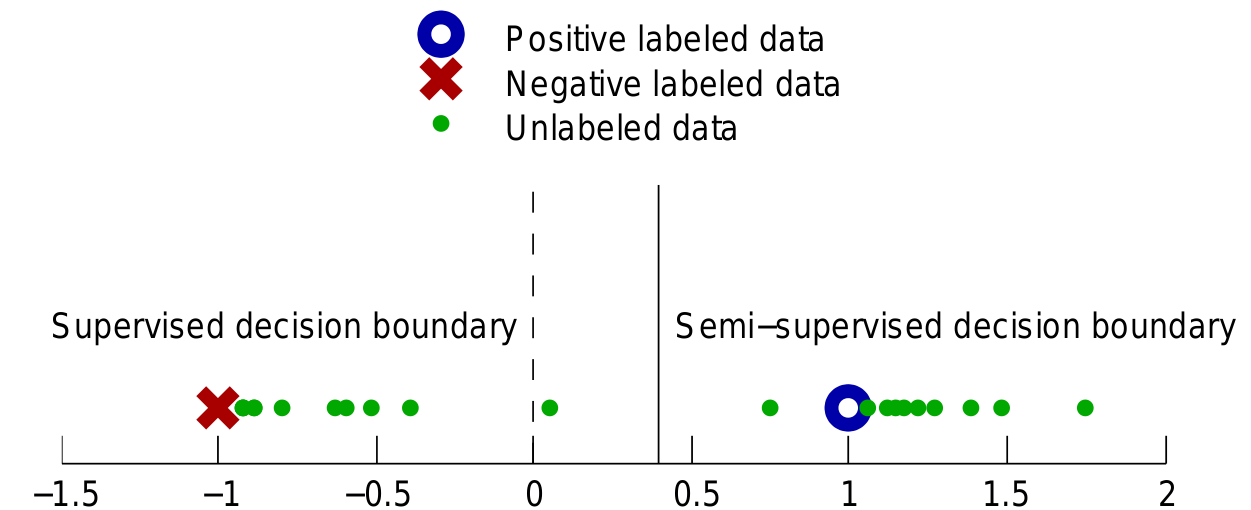
\includegraphics[width=.45\textwidth]{ssl-help}
  \end{center}
  \caption{Dados não-rotulados auxiliando a criar uma melhor fronteira de decisão. Fonte: \cite{zhu1}.}
  \label{fig:help}
\end{figure}

\begin{figure}[!h]
  \begin{center}
    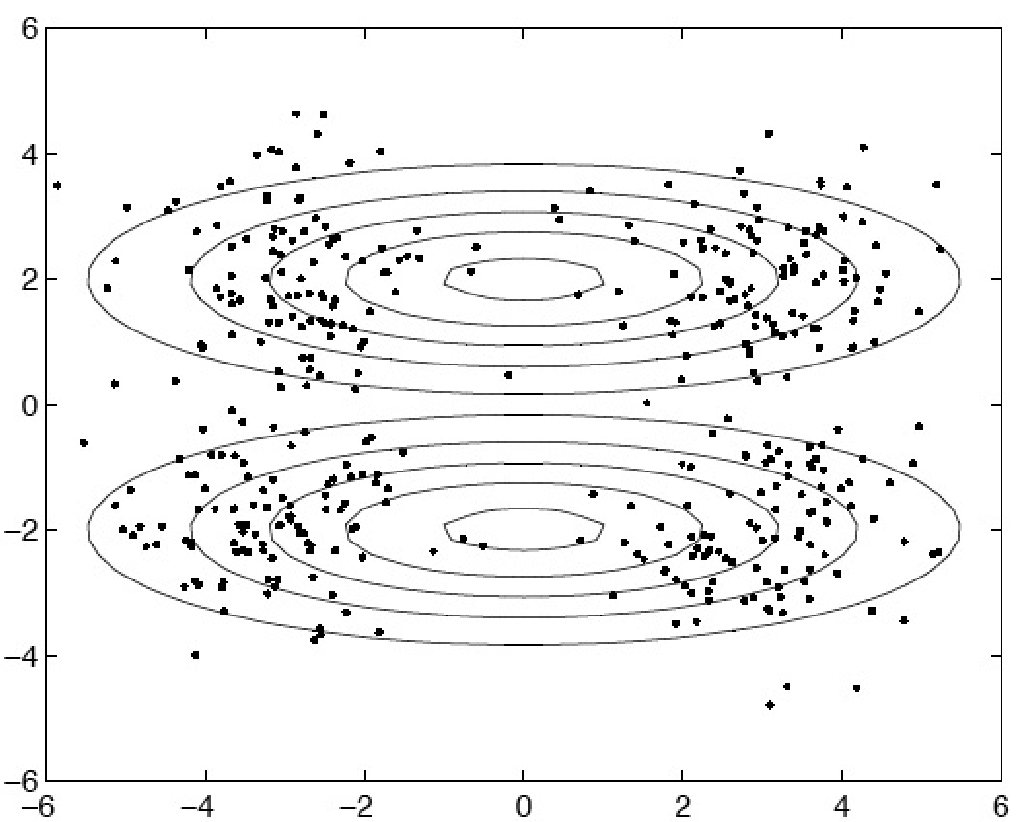
\includegraphics[width=.45\textwidth]{ssl-nhelp}
  \end{center}
  \caption{Dados não-rotulados atrapalhariam a correta separação das classes. Fonte: \cite{tub2008}.}
  \label{fig:nhelp}
\end{figure}


\subsubsection{Breve Histórico do Aprendizado Semi-Supervisionado}
Os primeiros trabalhos em CSS assumiam duas classes, cada uma com uma distribuição normal. Desta forma, os dados como um todo resultam em um \emph{modelo de mistura} (\emph{mixture model}). São necessárias somente de duas amostras rotuladas, uma de cada classe, para determinar completamente o modelo de mistura.

Uma variante é o \emph{self-training}: o classificador é treinado com os dados rotulados e depois aplicado aos não rotulados. Os pontos não rotulados que foram rotulados de forma mais confiante, são então adicionados ao conjunto de dados rotulados e então o classificador é treinado novamente. Este procedimento é chamado também de \emph{self-teaching} e \emph{bootstrapping}.

Ambos estes métodos são utilizados há muito tempo e continuam comuns devido à sua simplicidade conceitual e algorítmica.

Métodos mais recentes incluem o \emph{co-training} (em que dois classificadores utilizam partes disjuntas dos atributos de cada objeto e utiliza os novos objetos rotulados um do outro) e \emph{SVM transdutivo}.

Na última década, o aprendizado semi-supervisionado baseado em grafos atraiu grande atenção. Estes métodos iniciam-se com grafos cujos nós são os objetos rotulados e não rotulados e cujas arestas tem pesos que refletem a similaridade entre os objetos. Assume-se que objetos conectados por arestas de peso alto tendem a ter o mesmo rótulo e que os rótulos podem propagar-se pelo grafo. A seguir daremos uma definição e introdução mais formal sobre os grafos e sobre redes complexas.

\subsection{Grafos e Redes Complexas}
Está fora do escopo deste trabalho prolongar-se com a definição de grafos e redes complexas. Nesta parte é dado uma breve introdução e histórico sobre o tema. O estudo dos grafos é matéria da \emph{teoria dos grafos}.

Dito de forma direta, um grafo é uma representação abstrata de um conjunto de objetos no qual alguns destes objetos são ligados. Tais objetos são geralmente chamados de \emph{nós} ou \emph{vértices}. As ligações entre vértices são comumente chamadas de \emph{arestas}. Tipicamente, um grafo é visualmente representado por um conjunto de pontos ou bolas (os vértices) ligados por linhas (arestas).

Embora uma grande parte da teoria dos grafos seja elaborada apenas sobre esta estrutura básica descrita acima, existem diversos possíveis acréscimos estruturais. Provavelmente o mais importante é o de especificar uma direção para as arestas, resultando em \emph{arestas direcionadas}. A segunda característica diferencial de alguns grafos é a existência grandezas numéricas associadas às arestas, que resultam nas chamadas \emph{arestas com pesos}.

Outras características dos grafos são: mais de um tipo de aresta (possibilitando mais de uma aresta entre cada par de vértices); pesos associados aos nós; atributos diversos associados às arestas e aos nós (p.ex. cor); arestas incompletas; qualquer mistura de todas as características mencionadas acima.

Alguns grafos são clássicos, citamos alguns deles. Grafo regular é aquele no qual cada vértice tem o mesmo número de arestas. O grafo completo possui aresta entre qualquer par de vértices e também é chamado de \emph{click}. Um grafo conectado é aquele que apresenta um caminho de sucessão de arestas entre qualquer par de vértices. Grafo randômico é um grafo construído com uma probabilidade de se ter uma aresta entre dois vértices. Similarmente, um grafo randômico é aquele que exibe \emph{as mesmas características} que um grafo construído desta forma.

Formalmente falando, um grafo é um par ordenado $G=(V,E)$ composto de um conjunto de vértices $V$ e um conjunto $E$ de arestas, que são subconjuntos de $V$ com dois elementos. Estes são os grafos simples (com somente uma aresta possível entre cada par de vértices e sem aresta entre um vértice e ele mesmo) e não direcionado. Caso o conjunto $E$ seja composto de pares ordenados de elementos de $V$, o grafo é direcionado.

A medida mais comum de um grafo é o \emph{grau}, que é a quantidade de arestas ligadas a um vértice. Caso o grafo seja direcionado, podemos dividir o grau em duas quantidades: grau de entrada e grau de saída de um vértice. Caso o grafo tenha arestas com peso, pode-se falar em \emph{força} de um vértice que é a soma dos pesos das arestas ligadas ao vértice. Similarmente, podemos num grafo direcionado com peso, falar em força de entrada e força de saída de um vértice.

Antes de continuar com as medidas de um grafo, para o nosso caso é pertinente citar o que é uma \emph{rede complexa}. Dito de forma direta, uma rede complexa é um grafo com uma grande quantidade de vértices e arestas. Muitos pequisadores definem as redes complexas como sendo grafos de grandes dimensões que exibem características não triviais, isto é, que diferem de um grafo regular ou randômico. Esta definição é invalidada pelo fato de que se fala em rede complexa randômica e em rede complexa regular. Pode-se sim entender que a área de estudo das redes complexas se interessa pelos casos de redes complexas (comumente) encontrados na natureza que exibem características não triviais. 

Outra diferença entre as áreas de grafo e redes complexas é que enquanto a área de grafos tradicionalmente é vinculada à extração de propriedades matemáticas de grafos em geral ou com construções particulares, a área de redes complexas é marcada mais acentuadamente pela observação das redes complexas que representam fenômenos humanos ou naturais e suas divergências se comparadas às redes mais triviais (regulares e randômicas). Exemplos destas características peculiares são as conhecidas \emph{lei livre de escala} e \emph{lei de pequeno mundo}.

\subsubsection{Breve Histórico da Teoria dos Grafos e das Redes Complexas}
A estrutura de pontos e retas é tão simples que é difícil precisar quando foi utilizada pela primeira vez, se é que isso é possível. O artigo escrito por Leonhard Euler chamado "Konigsberg Bridge problem" é geralmente descrito como o primeiro trabalho tanto de topologia quanto de teoria dos grafos.

Mais de um século depois, Cayley estudou \emph{árvores} através de formas analíticas que surgiam do cálculo diferencial. Tais estudos tiveram grandes consequências para a química teórica e esta fusão entre química e grafos está no centro da nomenclatura comum utilizada para grafos.

Em particular, o nome \emph{grafo} foi introduzido por Sylvester em 1878 através de um artigo publicado na Nature.

No século XX a teoria dos grafos teve focos diferentes, passando pelo problema de coloração de grafos, topologia (em particular em conexão com a álgebra, p.ex. \emph{Lei de Kirchoff} para circuitos), e, por fim, por teorias probabilísticas.

Já adentrando o terreno das chamadas redes complexas, os artigos que demonstravam as características \emph{livre de escala} e de \emph{pequeno mundo} para grafos grandes representando estruturas da natureza~\cite{ferrer,barabasi} marcaram este novo grande interesse pela área.

Atualmente, as redes complexas são aplicadas com sucesso a diversas áreas~\cite{costaapp}, o que inclui neurociências~\cite{sporns}, física~\cite{pnas}, linguística~\cite{dorogo2} e ciência da computação~\cite{signature}, para citar simplesmente alguns casos.


\section{Aprendizado Semi-Supervisionado em Grafos}
Diversas técnicas de CSS baseada em grafos tem sido desenvolvidas e utilizadas. Citamos os seguintes métodos, de forma ilustrativa e sem a pretensão de obtermos uma lista completa: algorítmo de regularização ~\cite{reg}, mincut ~\cite{mincuts}, propagação de rótulo ~\cite{zhu3}, modelos de mistura e maximização de entropia \cite{zhu1}.

De especial importância é a forma de construção do grafo. Uma discussão detalhada sobre o assunto é encontrada no terceiro capítulo de ~\cite{zhu1}.

O resto desta seção é dedicado a explorar dois métodos e CSS com grafos, a saber a propagação de rótulo e o mincut.


\subsection{Propagação de Rótulo}
Estudamos aqui a propagação de rótulo em um grafo, onde o rótulo de um nó propaga aos nós vizinhos de acordo com as proximidades. Os rótulos dos dados rotulados são fixos, desta forma funcionam como fontes que emanam rótulos pelos dados não rotulados.

\subsubsection{Convenções e Exposição do Problema}
Sejam ${(x_1,y_1)...(x_l,y_l)}$ os dados rotulados, $y \in {1...C}$ com $C$ o número de classes e ${x_{l+1}...x_{l+u}}$ os dados não rotulados. Geralmente $l \ll u$. Seja $n = l + u$.

Note que $L$ e $U$ denotam os dados rotulados e não rotulados respectivamente.

É importante que as classes $C$ sejam conhecidas e que estejam presentes, cada uma, nos dados rotulados.

Este é um problema transdutivo, no qual devemos associar as classes dadas a cada um dos dados não rotulados. 

Criamos um grafo em que cada ponto é um dado, seja ele rotulado ou não rotulado. Para a criação das arestas fixamos o fato de que queremos dados similares com o mesmo rótulo. Já foram pensadas algumas formas diferentes de se fazer isso, a mais difundida assume um grafo totalmente conectado (há aresta entre qualquer par de nós). Cada aresta tem um peso, que reflete a similaridade entre os dados. Este peso pode ser calculado assim:

\begin{equation} \label{eqod}
        w_{ij} = exp( -\frac{\| x_i - x_j \|^2}{\alpha^2} )
\end{equation}

Onde $\alpha$ é um \emph{hiperparâmetro} regulador que deve ser testado em diferentes valores.

Os rótulos são propagados através das arestas. Pesos maiores permitem que os rótulos sejam propagados mais facilmente. Definimos a matriz probabilística de transição da seguinte forma:

\begin{equation}
  P_{ij} = P(i \rightarrow j) = \frac{w_{ij}}{\sum_{k=1}^{n}w_{ik}}
\end{equation}

Onde $P_{ij}$ é a probabilidade de transição do nó $i$ para o nó $j$ (passagem do rótulo). Também definimos a matriz de rótulos $Y_L$, $l \times C$, cuja \emph{iésima} linha possui $1$ na coluna correspondente à classe do dado $x_i$. 

A tarefa consiste em computar os rótulos dos nós todos (na verdade somente dos não rotulados). Seja $f$ uma matriz $n \times C$ em que cada linha pode ser interpretada como uma distribuição de probabilidade sobre os rótulos. Agora podemos seguir para o algoritmo (a inicialização de $f$ não é importante).

\subsubsection{O Algoritmo de Propagação de Rótulo}


O algoritmo de propagação de rótulo é o seguinte:

\begin{enumerate}
  \item Propague $f \leftarrow Pf$.
  \item Mantenha os dados rotulados iniciais $f_L = Y_L$.
  \item Repita do passo 1 até que o algoritmo convirja.
\end{enumerate}

No passo primeiro, todos os nós propagam o seu rótulo para os seus vizinhos. O segundo passo trata de assegurar que os rótulos dos nós inicialmente rotulados não sejam sobrescritos.

\subsubsection{Convergência}
O resultado interessante deste método é que ele não necessita do processo iterativo. Satisfeitas as condições de que todas as classes estejam presentes e de que cada componente conectado possua ao menos um dado rotulado, a convergência é segura.

Seja $f = \binom{f_L}{f_U}$. Como $f_L$ está fixo em $Y_L$, estamos somente interessados em $f_U$. Nós partimos $P$ em sub-matrizes rotuladas e não rotuladas:

\begin{equation}
  \begin{bmatrix}
    P_{LL} & P_{LU}
    \\P_{UL} & P_{UU}
  \end{bmatrix}
\end{equation}

Pode-se entender intuitivamente (e pode-se mostrar matematicamente) que este algorítmo é:

\begin{equation} \label{eq:inicio}
  f_U \leftarrow P_{UU}f_U + P_{UL}Y_L
\end{equation}

O que nos leva a:

\begin{equation}
  f_u = \lim_{n \rightarrow \infty}[(P_{UU})^n f_U^0 + (\sum_{i=1}^{n}(P_{UU})^{(i-1)})P_{UL}Y_L]
\end{equation}

onde $f_U^0$ é o valor inicial de $f_U$.

Mostraremos agora que, no primeiro termo, $(P_{UU})^n f_U^0 \rightarrow 0$. Lembrando que as linhas de $P$ estão normalizadas e $P_{UU}$ é uma sub-matriz de $P$, temos:

\begin{equation}
  \exists \; \gamma < 1 : \sum_{j = 1}^u(P_{UU})_{ij} \leq \gamma, \forall i = 1...u
\end{equation}

Portanto:

\begin{equation}
  \sum_j(P_{UU})_{ij}^n = \sum_j\sum_k(P_{UU})_{ik}^{(n-1)}(P_{UU})_{kj}
\end{equation}

\begin{equation}
  = \sum_k(P_{UU})_{ik}^{(n-1)}\sum_j(P_{UU})_{kj}
\end{equation}

\begin{equation}
  \leq \sum_k(P_{UU})_{ik}^{(n-1)}\gamma
\end{equation}

\begin{equation}
  \leq \gamma^n
\end{equation}

Podemos observar que a soma das linhas de $(P_{UU})^n$ converge para zero, o que significa que $(P_{UU})^nf_U^0 \rightarrow 0$. Note que o valor inicial $f_U^0$ não faz diferença.

Voltando à nossa condição inicial explicitada em (\ref{eq:inicio}) percebemos que temos o ponto fixo:

\begin{equation}
  f_u = (I - P_{UU})^{-1}P_{UL}Y_{L}
\end{equation}

Esta equação é, portanto, o único ponto fixo e a solução dada pelo nosso algoritmo iterativo. Isso nos permite resolver a questão de propagação de rótulo diretamente sem a propagação iterativa. 

Note que a solução é valida somente quando $I - P_{UU}$ é inversível. Esta condição é satisfeita intuitivamente quando cada componente conectado no grafo possui ao menos um ponto rotulado.

\subsubsection{Exemplos Ilustrativos}
Aqui demonstramos as propriedades do algorítmo de propagação de rótulos com dois bancos de dados artificiais. A Figura 1 mostra um banco de dados sintético com três bandas horizontais. Os pontos são uniformemente distribuidos das bandas. Existem 3 pontos rotulados (um para cada banda) e 178 dados não rotulados. Os dados foram rotulados utilizando-se \emph{k-nearest-neighbors} (com $k=1$) e o algoritmo de propagação de rótulos em grafos apresentado nesta monografia. 

Importante aqui é observar que o \emph{KNN} ignora os dados não rotulados e portanto a estrutura em bandas dos mesmos. Isso pode ser visto na Figura 2 em que parte dos dados de bandas diferentes assumem o rótulo do dados rotulado mais próximo, mas não o rótulo do dado rotulado que se encontra na mesma banda.

Isso é completamente resolvido no caso do algorítmo de propagação de rótulo. Foi utilizado $\alpha = 0.22$.

\begin{figure}[!h] \label{fig:horizontal1}
        \begin{center}
                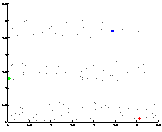
\includegraphics[width=0.35\textwidth]{prop1-dados}
        \end{center}
        \caption{Dados originais, 3 rotulados, 178 não rotulados.}
\end{figure}

\begin{figure}[!h] \label{fig:horizontal2}
        \begin{center}
                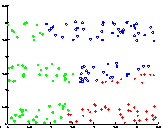
\includegraphics[width=0.35\textwidth]{prop1-dados-knn}
        \end{center}
        \caption{Dados rotulados utilizando-se knn.}
\end{figure}

\begin{figure}[!h] \label{fig:horizontal3}
        \begin{center}
                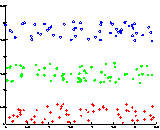
\includegraphics[width=0.35\textwidth]{prop1-dados-rotu}
        \end{center}
        \caption{Dados rotulados utilizando propagação de rótulos.}
\end{figure}

Já o o nosso segundo exemplo utiliza um banco de dados, também sintético, com duas classes espiraladas. O banco original, os 184 dados não rotulados e os 2 dados rotulados podem ser vistos na Figura 4.

Nas Figuras 6, 7 e 8 temos o mesmo comportamento do exemplo anterior. O \emph{KNN} não leva em consideração a distribuição dos dados, portanto as espirais acabam tendo elementos rotulados das duas maneiras. Já com a utilização da propagação de rótulos, cada espiral fica com sua própria classe.

\begin{figure}[!h] \label{fig:horizontal21}
        \begin{center}
                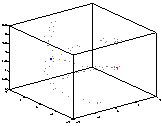
\includegraphics[width=0.35\textwidth]{prop2-dados}
        \end{center}
        \caption{Dados originais, 2 rotulados, 184 não rotulados.}
\end{figure}

\begin{figure}[!h] \label{fig:horizontal22}
        \begin{center}
                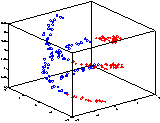
\includegraphics[width=0.35\textwidth]{prop2-dados-knn}
        \end{center}
        \caption{Dados espiralados rotulados utilizando-se knn.}
\end{figure}

\begin{figure}[!h] \label{fig:horizontal23}
        \begin{center}
                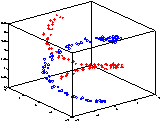
\includegraphics[width=0.35\textwidth]{prop2-dados-rotu}
        \end{center}
        \caption{Dados espiralados rotulados utilizando propagação de rótulos.}
\end{figure}

\subsection{Mincut}
Como a maior parte dos métodos de aprendizado semi-supervisionado, a idéia geral do método \emph{mincut} é associar rótulos aos dados não rotulados de forma a otimizar uma função objetivo. Para o caso do mincut, as funções objetivo são limitadas aos casos em que dependem somente das relações entre pares de nós.

O que torna este método especialmente atraente é a complexidade computacional que, para os casos em que o mincut pode ser aplicado, é polinomial e resulta no ótimo global. Portanto, mesmo com a perda da generalidade com relação ao EM (\emph{Expectation Maximization}) ou com o hill-climbing (que podem ser aplicados praticamente em qualquer caso), nos interessa a vantagem de calcular de fato o ótimo.

Neste caso temos a seguinte questão: quão interessantes são os casos em que podemos aplicar o mincut?

Vale notar que na literatura existe a seguinte relação: o mincut se relaciona aos algorítmos de vizinhos mais próximos assim como o SVM transdutivo se relaciona ao SVM padrão.

\subsubsection{Convenções e Exposição do Problema}
São dados os conjuntos de dados rotulados $L$ e não rotulados $U$. Sem perda de generalidade, assumimos que estamos interessados em uma classificação binária e denotamos por $L_+$ o conjunto de dados positivos em $L$ e por $L_-$ o conjunto de dados negativos em $L$. Os vértices em $L_+$ e $L_-$ serão denotados respectivamente $v_+$ e $v_-$ e serão chamados \emph{vértices de classificação}. Todos os outrso vértices serão chamados \emph{vértices de exemplo} ou simplesmente \emph{exemplos}.

\subsubsection{Algoritmo Mincut}
O algorítmo segue os seguintes passos:

\begin{enumerate}
  \item Construímos um grafo com pesos $G = (V,E)$, onde $V = L \cup U$ e $E \subseteq V \times V$. A cada aresta $e \in E$ é associado um peso $w(e)$.\footnote{Note que esta parte de montagem do problema não foi tida como parte do algoritmo no caso da propagação de rótulos, mas sim como parte das convenções e exposição do problema. No caso do mincut essa atribuição de pesos é bem menos resolvida.}

  \item Os vértices de classificação são conectados aos vértices de mesma classe com peso infinito. Ou seja, $w(v_1,v_2) = \infty, \forall \; v_1,v_2 \in L_+$ e $w(v_1,v_2) = \infty, \forall \; v_1,v_2 \in L_-$.

  \item Às arestas entre os vértices de exemplo são dados pesos com base em alguma relação entre os exemplos, tal qual a similaridade ou a distância entre eles. A função utilizada para atribuir peso às arestas dos exemplos é chamada (ao menos neste compêndio) de \emph{função de atribuição de pesos} e será denotado por $w$.

  \item Determinamos o conjunto de arestas com a menor soma de pesos que, se removidas, separam todos os $v_+$ dos $v_-$. Esta remoção é chamada de \emph{corte mínimo} do grafo e dá o nome ao método. Este corte mínimo parte o grafo em duas partes, às quais denominamos $V_+$ e $V_-$ nos quais todos os $v_+ \in V_+$ e todos os $v_- \in V_-$. Por completude, convencionamos que caso existam mais de um corte mínimo possível, escollhemos o que resulta em um $V_+$ menor.

  \item Por fim, rotulamos como positivos todos os vértices em $V_+$ e como negativos todos os vértives em $V_-$.
\end{enumerate}

A motivação principal para este algorítmo é que a dois vértices similares é associada uma aresta de peso alto e, portanto, estes provavelmente estarão no mesmo subconjunto de vértices. Isso é completamente concordante com a premissa básica da maioria dos algorítmimos de classificação: dados similares devem ter classes similares. 

Isso nos leva à função de atribuição de pesos $w$. Uma primeira e natural maneira de obtermos uma função de atribuição de pesos é através da distância euclidiana entre os objetos. Vértices com pequena distância entre si possuiriam grande peso e vértices com grande distância teriam pequeno peso. No caso de não termos diretamente como calcular esta distância euclidiana (p.ex. no caso de atributos não numéricos), então uma possibilidade é utilizar um algoritmo de aprendizado auxiliar que nos retorne as distâncias. O crucial aqui é o fato de que a forma de atribuição de pesos inflencia diretamente e fortemente o resultado e do algorítmo, assim como a sua qualidade.

\subsubsection{Calibragem}
O crítico neste algorítmo é sem dúvida a função de atribuição de pesos. Pode-se, inclusive, atribuir peso zero para a maior parte das arestas, selecionando somente as arestas de maior interesse para cada dado.

Das inumeráveis maneiras de se atribuir pesos, listamos a seguir duas formas principais de se formar as arestas, cada uma com as suas vantagens:

\begin{enumerate}
  \item {\bf Mincut-3} conectamos cada vértice a seu vizinho rotulado mais próximo e ao seus dois vizinhos mais próximos que não são o vizinho antes escolhido. Esta conexão forçada com o rotulado mais próximo tem o intuito de evitar a formação de componentes isolados.

  \item {\bf Mincut-$\delta$} utilizando-se da métrica do espaço das variáveis, se a distância entre dois dados for menos que um dado limiar denotado por $\delta$, conectamos os vértices correspondentes por uma aresta. A melhor escolha de $\delta$ pode variar bastante dependendo das intensões e do banco de dados. Segue algumas alternativas:
  \begin{itemize}
    \item No {\bf Mincut-$\delta_0$}, escolhemos o $\delta$ máximo para o qual o grafo tem um corte de valor zero.

    \item No {\bf Mincut-$\delta_\frac{1}{2}$}, utilizamos um valor para $\delta$ em que o tamanho do maior componente conectado no grafo possui metade dos dados.

    \item No {\bf Mincut-$\delta_{opt}$}, escolhemos o valor de $\delta$ que apresenta o menor erro. Este $\delta$ é estabelecido depois de testes e serve como um valor de referência para o estudo do desempenho de outros valores de $\delta$.
  \end{itemize}
\end{enumerate}


\subsubsection{Discussão}
Os resultados obtidos pela utilização do mincut são bastante relacionados aos obtidos com a utilização do \emph{kNN}\footnote{Resultado levantado pela utilização do LOOCV (\emph{leave-one-out cross-validation}.}.

Este algorítmo também não está livre de problemas. Alguns podem ser notados com clareza. Pode-se ter problemas caso tenhamos pouquíssimos exemplos rotulados (ou muito localizados) e muitos exemplos não rotulados. Neste caso o algorítmo pode separar quase a totalidade dos dados para uma só  classe. Por exemplo, se temos somente um dado positivo e outro negativo e conectamos cada vértice aos seus três vizinhos mais próximos com arestas de peso 1, o corte em que temos somente o vértice posivo na classe dos positivos tem custo 3.

Outro problema em potencial pode surgir no caso em que o grafo é esparço o suficiente para ter um certo número de componentes não conectados\footnote{Por exemplo, no caso de se utilizar kNN, uma parte dos dados pode criar uma componente isolada.}. O algorítmo de mincut deverá então escolher arbitrariamente qual rótulo associar a todo o compontente. Desta forma podemos entender que a função de atribuição de peso deve ser escolhida cuidadosamente de forma a não permitir que isso aconteça.

\begin{figure*}[ht] \label{fig:hori}
        \begin{center}
                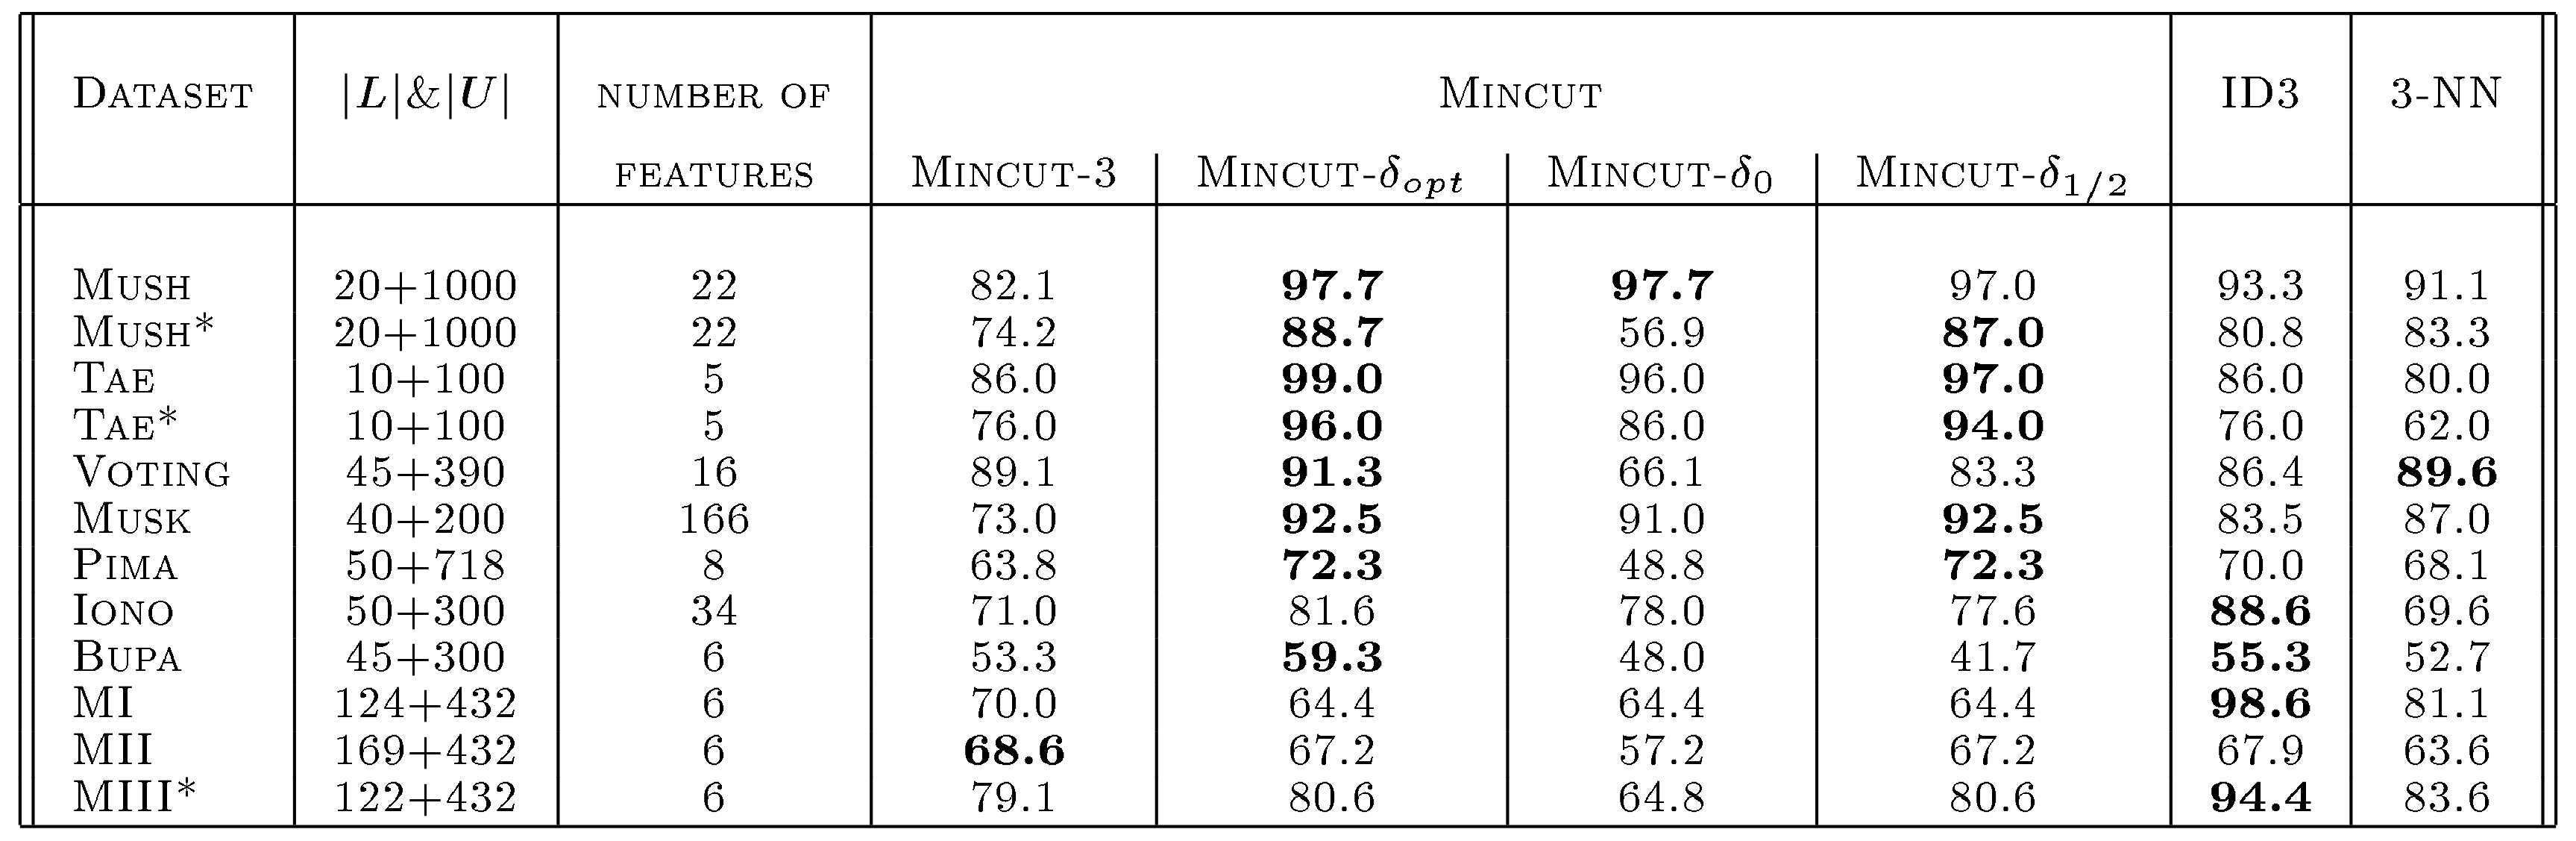
\includegraphics[width=1.0\textwidth]{mincut-comp}
        \end{center}
        \caption{Mincut com alguns valores para $\delta$ e comparação com outros métodos.}
\end{figure*}

\begin{figure} \label{fig:delta}
        \begin{center}
                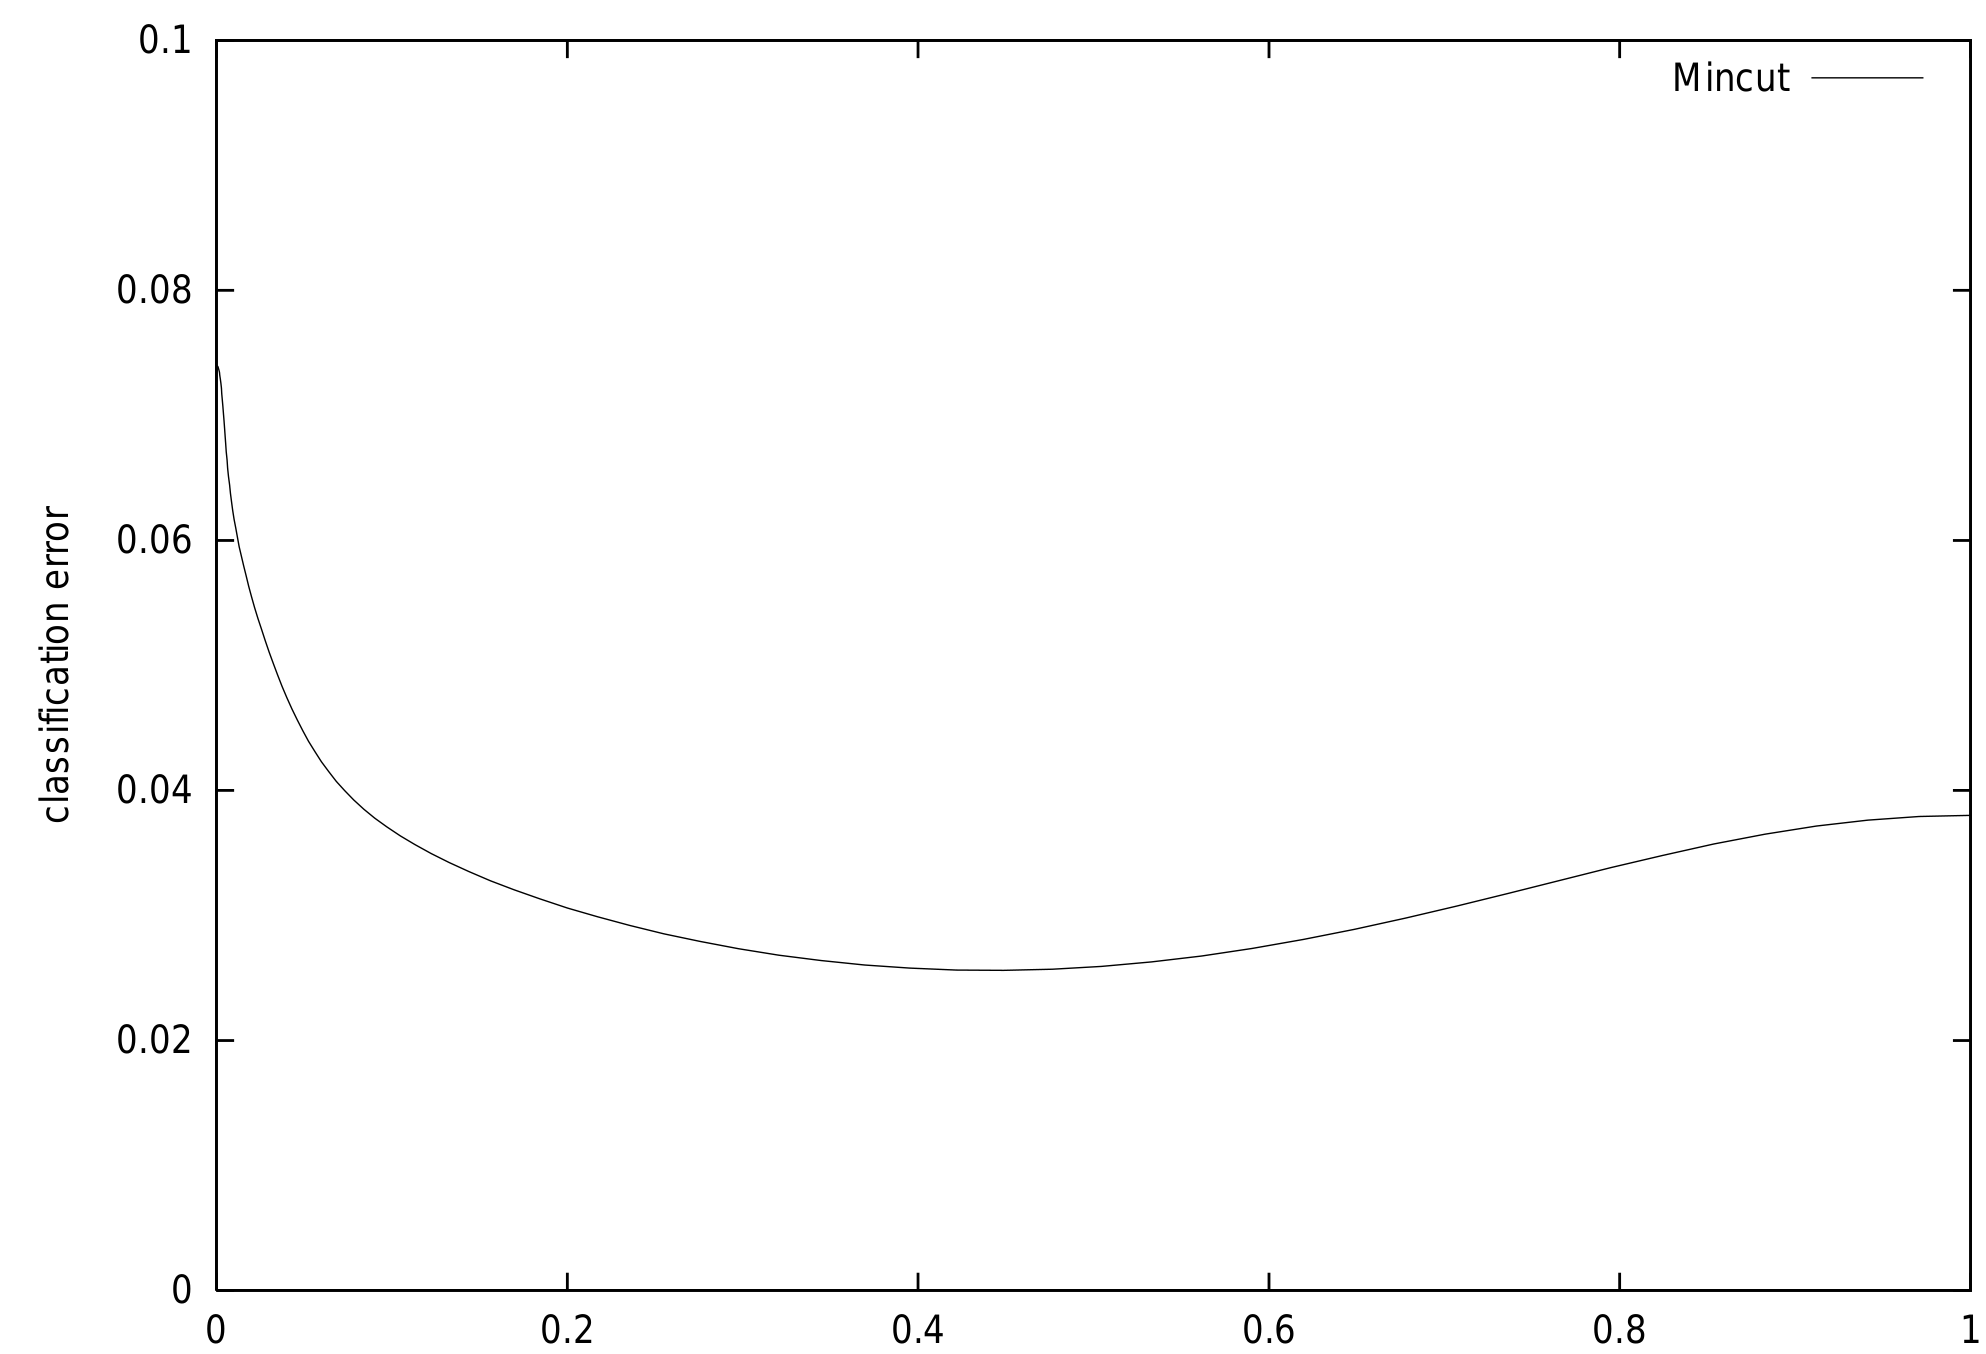
\includegraphics[width=.45\textwidth]{mincut-delta}
        \end{center}
        \caption{Variação do erro com o Delta.}
\end{figure}

\begin{figure} \label{fig:mincut-l}
        \begin{center}
                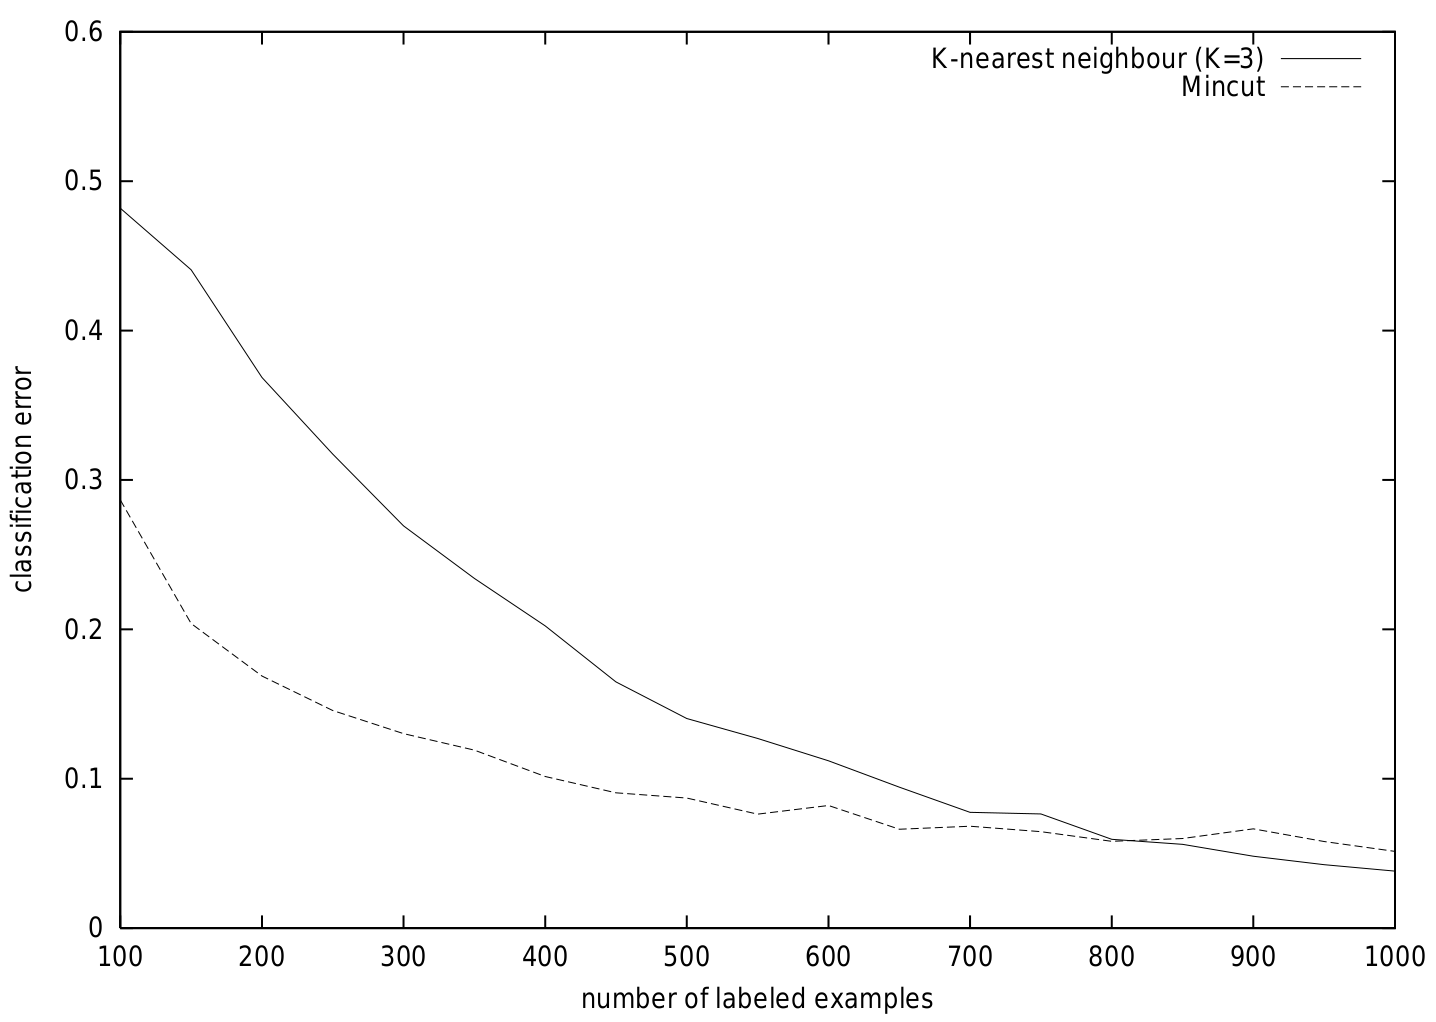
\includegraphics[width=.45\textwidth]{mincut-erro-l}
        \end{center}
        \caption{Comparação do erro entre mincut e kNN com a variação de exemplos rotulados $\delta_{opt}$.}
\end{figure}

\begin{figure} \label{fig:mincut-l}
        \begin{center}
                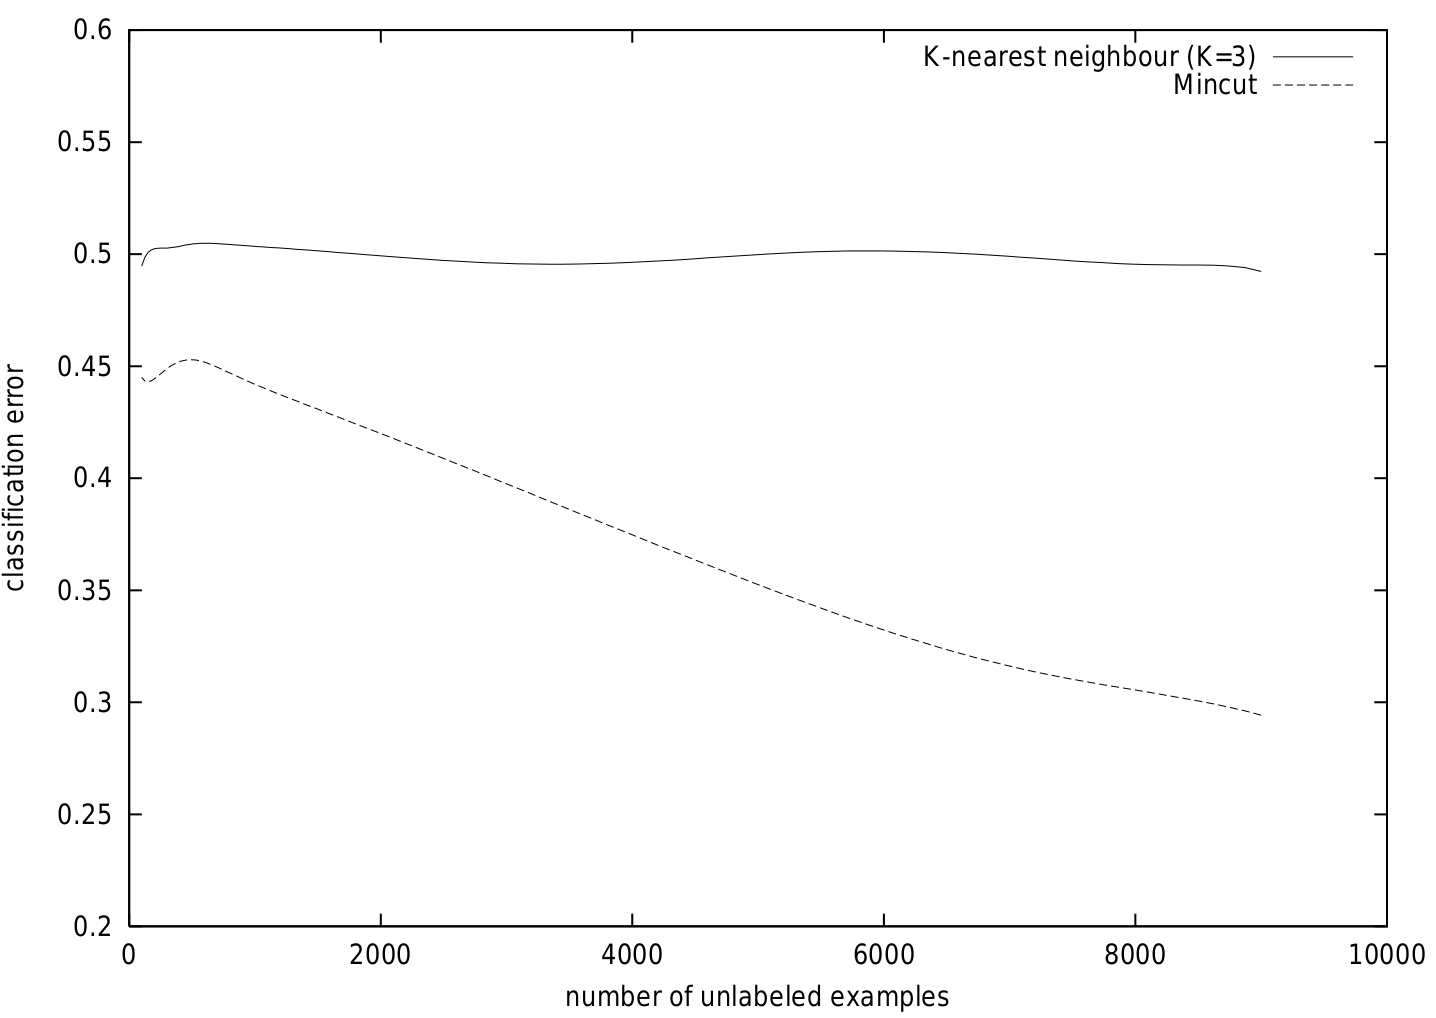
\includegraphics[width=.45\textwidth]{mincut-erro-u}
        \end{center}
        \caption{Comparação do erro entre mincut e kNN com a variação de exemplos não rotulados $\delta_{opt}$.}
\end{figure}


\section{Conclusão}
A utilização de dados não rotulados para CSS é de grande utilidade quando os dados rotulados são poucos ou custosos. Também pode-se utilizar com segurança CSS quando as classes estão clusterizadas entre si.

O método de propagação de rótulo assegura uma classificação que segue a distribuição das amostras, não somente a proximidade de um dado a outro rotulado, como no caso do kNN. Já o método do mincut apresenta a dificuldade de seleção do método de interconexão dos dados, i.e. da distribuição das arestas. Mesmo assim, segundo os resultados que temos, ele apresenta melhor performance que o tradicional kNN para a maioria dos casos. Isso se deve também à utilização da estrutura dos dados para a classificação geral. 

\begin{thebibliography}{}


\bibitem[\protect\citename{Zhu, X. and Lafferty, J. and Rosenfeld, R.}2005]{zhu1}
Zhu, X. and Lafferty, J. and Rosenfeld, R.
\newblock 2005.
\newblock {Semi-supervised learning with graphs}.
\newblock {\em Unpublished doctoral dissertation}.

\bibitem[\protect\citename{Zhu, X.}2007]{zhu2}
Zhu, X.
\newblock 2006.
\newblock {Semi-supervised learning literature survey}.
\newblock {\em Citeseer}.

\bibitem[\protect\citename{Zhu, X. and Ghahramani, Z.}2003]{zhu3}
Zhu, X. and Ghahramani, Z.
\newblock 2002.
\newblock {Learning from labeled and unlabeled data with label propagation}.
\newblock {\em Citeseer}.

\bibitem[\protect\citename{Blum, A. and Chawla, S.}2001]{mincuts}
Blum, A. and Chawla, S.
\newblock 2001.
\newblock {Learning from labeled and unlabeled data using graph mincuts}.

\bibitem[\protect\citename{Belkin, M. and Matveeva, I. and Niyogi, P.}2004]{ferrer}
Belkin, M. and Matveeva, I. and Niyogi, P.
\newblock 2004.
\newblock {Regularization and Semi-supervised Learning on Large Graphs}.
% \newblock {\em Proceedings of the Royal Society of London B}, 268:2261.

\bibitem[\protect\citename{Müller, K. R. and Zien, A.}2008]{tub2008}
Müller, K. R. and Zien, A.
\newblock 2008.
\newblock {Semi-Supervised Learning}.

\bibitem[\protect\citename{Chapelle, O. and Sch{\\"o}lkopf, B. and Zien, A.}2006]{sslbook}
Chapelle, O. and Sch{\\"o}lkopf, B. and Zien, A.
\newblock 2006.
\newblock {Semi-supervised learning}.
\newblock {\em Citeseer}.

\bibitem[\protect\citename{Ferrer i Cancho and Sole}2001]{ferrer}
R. Ferrer i Cancho and R. V. Sole.
\newblock 2001.
\newblock {The small world of human language}.
\newblock {\em Proceedings of the Royal Society of London B}, 268:2261.

\bibitem[\protect\citename{Newman}2003]{newman}
M. E. J. Newman. 
\newblock 2003.
\newblock {The Structure and Function of Complex Networks}.
\newblock {\em SIAM Review}, 45:167--256.

\bibitem[\protect\citename{Albert and Barabasi}2002]{barabasi}
R. Z. Albert and A.L. Barabasi. 
\newblock 2002.
\newblock {Statistical Mechanics of Complex Networks}.
\newblock {\em Rev. Modern Phys.}, 74:47--97.

\bibitem[\protect\citename{Costa \bgroup et al.}2008]{costaapp}
L. F. da Costa, O. N. Oliveira Jr., G. Travieso, F. A. Rodrigues, P. R. Villas Boas, L. Antiqueira, M. P. Viana, L. E. C. da Rocha. 
\newblock 2008.
\newblock {Analyzing and Modeling Real-World Phenomena with Complex Networks: A Survey of Applications}.
\newblock {\em arXiv} 0711.3199.

\bibitem[\protect\citename{Sporns}2002]{sporns}
O. Sporns. 
\newblock 2002.
\newblock {Network analysis, complexity, and brain function}.
\newblock {\em Complexity}, 8(1):56--60.

\bibitem[\protect\citename{Gfeller}2007]{pnas}
D. Gfeller, P. LosRios, A. Caflisch and F. Rao.
\newblock 2007.
\newblock {Complex network analysis of free-energy landscapes}.
\newblock {\em Proceedings of the National Academy of Science USA}, 104 (6):1817--1822

\bibitem[\protect\citename{Dorogovtsev and Mendes}2001]{dorogo2}
S. N. Dorogovtsev and J. F. F.Mendes.
\newblock 2001.
\newblock {Language as an evolving word web}.
\newblock {\em Proceedings of the Royal Society of London B}, 268:2603.

\bibitem[\protect\citename{Moura \bgroup et al.}2003]{signature}
A. P. S. de Moura, Y. C. Lai and A. E. Motter.
\newblock 2003.
\newblock {Signatures of small-world and scale-free properties in large computer programs}.
\newblock {\em Physical Review E}, 68(1):017102.

\bibitem[\protect\citename{Belkin, M. and Matveeva, I. and Niyogi, P.}2004]{reg}
Belkin, M. and Matveeva, I. and Niyogi, P..
\newblock 2004.
\newblock {Regularization and semi-supervised learning on large graphs}.
\newblock {\em Learning theory, Springer}, 624--638.



% \bibitem[\protect\citename{John and Langley}1995]{bayes}
% G. H. John and P. Langley.
% \newblock 1995.
% \newblock {Estimating Continuous Distribution in Bayesian Classifiers}.
% \newblock {\em 11 Conference on Uncertainty in Artificial Intelligence}, 338--345. 
% 
% \bibitem[\protect\citename{Kohavi}1995]{cross}
% R. Kohavi.
% \newblock 1995.
% \newblock {A study of cross-validation and bootstrap for accuracy estimation and model selection}.
% \newblock {\em Proceedings of the Fourteenth International Joint Conference on Artificial Intelligence 2}, 12:1137-1143. 

\end{thebibliography}

\end{document}







